%%%%%%%%%%%%%%%%%%%%%%%%%%%%%%%%%%%%%%%%%%%%%%%%%%%%%%%%%%%%%%%%%%%%%%%%%%%%%%%%
%2345678901234567890123456789012345678901234567890123456789012345678901234567890
%        1         2         3         4         5         6         7         8

\documentclass[letterpaper, 10 pt, conference]{ieeeconf}  % Comment this line out if you need a4paper

%\documentclass[a4paper, 10pt, conference]{ieeeconf}      % Use this line for a4 paper

\IEEEoverridecommandlockouts                              % This command is only needed if 
                                                          % you want to use the \thanks command

\overrideIEEEmargins                                      % Needed to meet printer requirements.

%In case you encounter the following error:
%Error 1010 The PDF file may be corrupt (unable to open PDF file) OR
%Error 1000 An error occurred while parsing a contents stream. Unable to analyze the PDF file.
%This is a known problem with pdfLaTeX conversion filter. The file cannot be opened with acrobat reader
%Please use one of the alternatives below to circumvent this error by uncommenting one or the other
%\pdfobjcompresslevel=0
%\pdfminorversion=4

% See the \addtolength command later in the file to balance the column lengths
% on the last page of the document

% The following packages can be found on http:\\www.ctan.org
%\usepackage{graphics} % for pdf, bitmapped graphics files
\usepackage{graphicx}
%\usepackage{epsfig} % for postscript graphics files
%\usepackage{mathptmx} % assumes new font selection scheme installed
%\usepackage{times} % assumes new font selection scheme installed
%\usepackage{amsmath} % assumes amsmath package installed
%\usepackage{amssymb}  % assumes amsmath package installed


\newtheorem{theorem}{Theorem}
\newtheorem{lemma}{Lemma}
\newtheorem{definition}{Definition}
\newtheorem{remark}{Remark}
\newtheorem{assumption}{Assumption}
\newtheorem{property}{Property}
\newtheorem{corollary}{Corollary}
\newtheorem{proposition}{Proposition}

\title{Distributed Command Filtered  Robust Tracking Control of Wave-Adaptive Modular Vessel with Uncertainty}

\author{Md. Nur-A-Adam Dony, Mohammad Rafat,  and Wenjie Dong$^*$% <-this % stops a space
\thanks{*Corresponding author: W. Dong 
        ({\tt\small wenjie.dong@utrgv.edu})}% <-this % stops a space
\thanks{Md. Nur-A-Adam Dony, Mohammad Rafat, and Wenjie Dong are with Department of Electrical and Computer Engineering, the University of Texas Rio Grande Valley,
Edinburg, TX 78539, USA}%
}


\begin{document}
\maketitle
\begin{abstract} This paper considers formation control of multiple wave-adaptive-modular vessels (WAM-Vs) with the aid of neighbors' information when there are parametric uncertainty and non-parametric uncertainty in the dynamics of each WAM-V. With the aid of backstepping techniques,  distributed robust tracking controllers are proposed. To avoid calculation of the derivative of signals, distributed command filtered controllers are also proposed.  
 Simulation results show the effectiveness of the proposed controllers.
\end{abstract}

\section{Introduction}

A Wave-Adaptive Modular Vessel (WAM-V) is an underactuated system. There are fewer control inputs than the numbers of the degree of freedom. Control of a WAM-V is challenging due to its underactuated nature. In oceans, there are always unknown currents applied to a WAM-V. Therefore, in the model of a WAM-V, there are always disturbances.
Considering the complexity of tasks, robustness and flexibility of multiple WAM-Vs, coordination of multiple systems has been an important mission. In this paper, we considered formation control of multiple WAM-Vs with uncertainty. It is assumed that there is parametric uncertainty and non-parametric uncertainty in the model of each WAM-V and the information of the leader WAM-V is available only to a portion of the follower WAM-Vs.



Cooperative control of multiple agents has received
considerable attention in recent years.  Various
methods have been proposed, which include behavior-based method
\cite{law03}, virtual structure based method \cite{bea01},
leader-follower method
 \cite{tan04}, artificial potentials based method
  \cite{leo01},
graph theory based method
\cite{dongFarrell}.

Formation control of surface vessels is particularly interesting and
has many applications in practice. For example, several autonomous vessels trace a target and enclose it; several vessels search a target in a large water area cooperatively; and several vessels with some sensors on them, monitor a large area cooperatively for security, etc.
One important type of
formation control  is to design cooperative control
laws such that a group of surface vessels converges to a  geometric
pattern which is moving along a desired trajectory or path. This formation control problem is complicated due to the nonlinearity and underactuated features of 
the dynamics of each surface vehicle.  In
\cite{arr06,arr061}, applications of the null-space-based behavioral
control to a fleet of marine surface vessels were discussed.
Cooperative controls which could achieve multiple tasks were
proposed. In \cite{bre06}, a planar formation control problem of
multiple agents was considered. A guided formation control scheme
was developed by combining guidance laws with synchronization
algorithms and collision avoidance techniques. In \cite{ihl06},
robust formation control of marine craft was considered. Cooperative
control laws were proposed with the aid of a set of inter-body
constraint functions and Lagrangian multipliers.
 In \cite{agu06}, the formation control along a desired path was
 discussed. Decentralized controllers were proposed with the aid of
 Lyapunov-based techniques and graph
theory results.  In \cite{bor06}, cross-track formation control of
underactuated 3-DOF surface vessels was considered. Decentralized
controllers with two blocks were proposed such that a group of
vessels asymptotically converged to a desired formation which
followed a given straight-line path with a given forward speed
profile. In papers \cite{arr06,arr061,bre06,ihl06}, the controlled
systems are assumed to be fully actuated. In \cite{Xia2019}, dynamic positioning of multiple surface vessels subject to unknown time-varying environmental disturbances and input saturation was considered. Distributed controllers were proposed with the aid of disturbance observer and dynamic surface control technique.


In this paper, we consider formation control of multiple WAM-Vs with uncertainty and a leader vehicle. Distributed robust controllers are proposed with the aid of adaptive backstepping techniques. 
The proposed control laws ensure that the formation errors and the tracking errors exponentially converge to zero. To reduce the computation load in controller design, distributed command filtered controllers are proposed.  To verify the effectiveness of the proposed
cooperative control laws, simulation results are presented.


\section{Problem statement }
\label{sec2}


\subsection{WAM-V Modeling}
\label{model}

It is considered a group of $m$ wave-adaptive modular vessels (WAM-Vs). Each WAMV has  two propellers in its pontoons. With the aid of the results in \cite{fos94},
the kinematics of the $j$-th WAM-V can be written as
\begin{eqnarray}
\dot{x}_j&=&u_j\cos\psi_j  -v_j\sin\psi_j \label{e1a}\\
\dot{y}_j&=&u_j\sin\psi_j +v_j\cos\psi_j \label{e1b}\\
\dot{\psi}_j&=&r_j \label{e1c}
\end{eqnarray}
where $(x_j, y_j)$ denotes the coordinates of the center of the WAM-V in the earth-fixed frame, $\psi_j$ is the
orientation of the WAM-V, and $u_j$, $v_j$ and $r_j$ are the
velocities of the WAM-V in surge, sway and yaw,
respectively.  For simplicity of analysis, it is assumed that the $j$th WAM-V has port/starboard and fore/aft symmetry and the motion in heave, roll and pitch can be neglected. The dynamics of the $j$th WAM-V can be
written as (\cite{fos94})
\begin{eqnarray}
&&m_{1j}\dot{u}_j-m_{2j}v_jr_j+
d_{1j}u_j+D_{1j}=F_{Lj}+F_{Rj} \label{e2a}\\
&&m_{2j}\dot{v}_j+m_{1j}u_jr_j+d_{2j}v_j+D_{2j}=0 \label{e2b}\\
&&m_{3j}\dot{r}_j-(m_{1j}-m_{2j})u_jv_j+d_{3j}r_j+D_{3j}\nonumber\\
&&=
L_j(F_{Lj}-F_{Rj})
 \label{e2c}
\end{eqnarray}
where $m_{ij}(>0)$  and $d_{ij}(>0)$  for $i=1,2,3$ are (effective)
 inertia and  hydrodynamic damping of the WAM-V,
respectively; $L_j$ is the moment arm of the forces with respect to the center of geometry and mass of the WAM-V, which are assumed to coincide; $D_{ij}$ is un-modeled dynamics and disturbance, and $F_{Lj}$ and $F_{Rj}$ are the force generated by the propellers. 


For control purpose, each WAM-V knows its own state and
the states of its neighbors by wireless communication or sensors. If each WAM-V is considered as a node, the communications between WAM-Vs
can be described by a directed graph (i.e., digraph) ${\cal G}=\{{\cal V},{\cal E}\}$,
where ${\cal V}=\{1,2,\ldots,m\}$ is a node set, ${\cal E}$ is an
edge set with elements $(i,j)$ which describes the communication
from node $i$ to node $j$. If the state of node $i$ is available
to node $j$, there is an edge $(i,j)$ in ${\cal E}$, and vice
versa. Node $i$ is a {\em neighbor} of node $j$ if the
state of node $i$ is available to node $j$. Since communication
is directional, $(i,j)$ is an ordered pair, which means that
$(i,j)\in {\cal E}$ does not mean $(j,i)\in {\cal E}$. For node
$j$, the indexes of its neighbors form a set which is denoted by
${\cal N}_j$. Therefore, the available states to node $j$ are the state of node $j$ and the state of node $i$ for
all $i\in{\cal N}_j$.  A directed path
in a digraph is an ordered sequence of vertices such that any ordered pair of
vertices appearing consecutively in the sequence is an edge of the digraph.
Node $i$ is reachable to node $j$ ($j\not=i$) if there exists a directed path from node $i$ to node $j$.
For more terminology on graph theory, interested
readers may refer to \cite{chu97,mer98}.

\subsection{Problem Statement}


In the dynamics (\ref{e2a})-(\ref{e2c}), the inertia parameters $m_{ij}$ and $d_{ij}$ are not exactly known in practice. 

It is given a leader WAM-V which moves along a smooth trajectory $(x_0(t),y_0(t))$.
The leader WAM-V is labeled as node $0$. The $m$ WAM-Vs in (\ref{e1a})-(\ref{e1c}) are called the follower WAM-Vs.
The state of the leader WAM-V is available to some of the follower WAM-Vs. The communication between $m$ follower WAM-Vs and the leader WAM-V is described by a digraph ${\cal G}^e=\{{\cal V}^e,{\cal E}^e\}$ with a node set ${\cal V}^e=\{0,1,2,\ldots,m\}$. For node $j$ ($0\leq j\leq m$), its neighbor set is denoted as ${\cal N}_j^e$.  Node $0$ is said to be globally reachable if node $0$ is reachable to node $j$ for $1\leq j\leq m$. In this paper, the following assumption is made on the communication digraph ${\cal G}^e$.

\begin{assumption}
In the communication digraph ${\cal G}^e$, node $0$ is globally reachable.
\label{ass1}
\end{assumption}

It is also given a desired geometric pattern ${\cal P}$ defined by constant
vectors $[p_{jx},p_{jy}]^\top (1\leq j\leq m)$ which satisfy
$ \sum^m_{j=1}p_{jx}=0$ and $\sum^m_{j=1}p_{jy}=0.$
We consider the following formation control problem.


{\em Formation Control Problem:} Design a controller $(F_{Lj},F_{Rj})$ for $j$-th follower WAM-V
based on its neighbors' state information such that
\begin{eqnarray}
\lim_{t\rightarrow\infty}\left[\begin{array}{c} x_i-x_j\\
y_i-y_j\end{array}\right]=\left[\begin{array}{c}
p_{ix}-p_{jx}\\
p_{iy}-p_{jy}\end{array}\right], 1\leq i,j\leq m \label{goal1}\\
\lim_{t\rightarrow\infty}\sum^m_{j=1}\left(\frac{x_j}{m}-x_0\right)=0\makebox[4cm]{}\label{goal2}\\
\lim_{t\rightarrow\infty}\sum^m_{j=1}\left(\frac{y_j}{m}-y_0\right)=0\makebox[4cm]{}\label{goal3}
\end{eqnarray}


In the above problem, eqn. (\ref{goal1}) means that
$m$ follower WAM-Vs come into the desired geometric
pattern ${\cal P}$. Eqn. (\ref{goal2})-(\ref{goal3}) mean that the centroid of $m$ follower WAM-Vs follows the leader WAM-V.


\section{Distributed Robust Controller Design}
\label{sec4}

 It is assumed that the nominal values of $m_{ij}$ and $d_{ij}$ are $\bar{m}_{ij}$ and $\bar{d}_{ij}$, respectively. The errors between the nominal values and the real values are bounded by known constants, i.e.,
$|m_{1j}-\bar{m}_{1j}|\leq \rho_{1j}$, $|m_{2j}-\bar{m}_{2j}|\leq \rho_{2j}$, $|m_{3j}-\bar{m}_{3j}|\leq \rho_{3j}$,
$|d_{1j}-\bar{d}_{1j}|\leq \rho_{4j}$, $|d_{3j}-\bar{d}_{3j}|\leq \rho_{5j}$,  $\left|D_{1j}\right|\leq \rho_{6j}$, and
$\left|D_{3j}\right|\leq \rho_{7j}$, 
where $\rho_{ij}$ ($1\leq i\leq 7$) are known.
The system in (\ref{e1a})-(\ref{e2c}) has a cascade structure. We will take this advantage and design a  distributed controller for the $j$-th WAM-V with the aid of backstepping techniques \cite{krs95}. 

$\bullet$ {\bf Step 1:} For system $j$, the weighted average of its
neighbors information is defined as
\begin{eqnarray}
\zeta_{1j}=\frac{\displaystyle{\sum_{i\in{\cal N}^e_j}}a_{ji}(x_i-p_{ix})}{\displaystyle{\sum_{i\in{\cal N}^e_j}}a_{ji}},~~
\zeta_{2j}=\frac{\displaystyle{\sum_{i\in{\cal
N}^e_j}}a_{ji}(y_i-p_{iy})}{\displaystyle{\sum_{i\in{\cal
N}^e_j}}a_{ji}}\label{gzeta2j}
\end{eqnarray}
where ${\cal N}^e_j$ is the neighbor set of node $j$ in the digraph
${\cal G}^e$,  $a_{ji}$ is a positive constant for $j=1,2,\ldots,m$.
In the system  (\ref{e1a})-(\ref{e1b}), we consider $u_j\cos\psi_j$
and $u_j\sin\psi_j$ as virtual control inputs and design tracking
controllers such that
\begin{eqnarray}
\lim_{t\rightarrow\infty}(x_j(t)-p_{jx}-\zeta_{1j}(t))=0\label{gg1}\\
\lim_{t\rightarrow\infty}(y_j(t)-p_{jy}-\zeta_{2j}(t))=0.\label{gg2}
\end{eqnarray}
 For convenience, we
let
\begin{eqnarray}
u_j\cos\psi_j=\eta_{1j},~~
u_j\sin\psi_j=\eta_{2j}.\label{gtp433}
\end{eqnarray}
where $\eta_{1j}$ and $\eta_{2j}$ will be chosen later. Let the
tracking error
\begin{eqnarray}
e_{*j}=\left[\begin{array}{c}e_{1j}\\
e_{2j}\end{array}\right]=\left[\begin{array}{c}x_j-p_{jx}-\zeta_{1j}\\
y_j-p_{jy}-\zeta_{2j}\end{array}\right] \label{ge_def}
\end{eqnarray}
then
\begin{eqnarray}
\dot{e}_{*j}=\left[\begin{array}{c}\eta_{1j}\\
\eta_{2j}\end{array}\right]+\left[\begin{array}{c}-\sin\psi_j\\
\cos\psi_j\end{array}\right]v_j
-\left[\begin{array}{c}\dot{\zeta}_{1j}\\
\dot{\zeta}_{2j}\end{array}\right]\label{ge901}
\end{eqnarray}
(\ref{ge901}) can be considered as a linear system with
perturbations. Stabilizing controllers can be designed as
\begin{eqnarray}
\eta_{1j}&=&-a_{jj}e_{1j}+v_j\sin\psi_j-\frac{\rho_{x}e_{1j}}{\sqrt{e^2_{1j}+h(t)}}\label{geta1j} \\
\eta_{2j}&=&-a_{jj}e_{2j}-v_j\cos\psi_j-\frac{\rho_{y}e_{2j}}{\sqrt{e^2_{2j}+h(t)}}\label{geta2j}
\end{eqnarray}
where $a_{jj}=\sum_{i\in{\cal N}^e_j}a_{ji}$, $\rho_{x}$ and
$\rho_y$ are sufficiently large constants, $h(t)>0$, and $h(t)$
exponentially converges to zero.

To verify that the proposed virtual controller
(\ref{geta1j})-(\ref{geta2j}) ensures that (\ref{gg1})-(\ref{gg2})
hold, we substitute the virtual controller
(\ref{geta1j})-(\ref{geta2j}) to (\ref{e1a})-(\ref{e1b}) and have
\begin{eqnarray}
\dot{x}_j=-\sum_{i\in{\cal N}^e_j}a_{ji}(x_j-p_{jx}-x_i+p_{ix})-\frac{\rho_xe_{1j}}{\sqrt{e^2_{1j}+h}}\label{gtp1010}\\
\dot{y}_j=-\sum_{i\in{\cal
N}^e_j}a_{ji}(y_j-p_{jy}-y_i+p_{iy})-\frac{\rho_ye_{2j}}{\sqrt{e^2_{2j}+h}}.\label{gtp1013}
\end{eqnarray}
Define $\tilde{x}_j=x_j-p_{jx}-x_0$ and $\tilde{y}_j=y_j-p_{jy}-y_0$
where $p_{0x}=p_{0y}=0$, we have
\begin{eqnarray}
\dot{\tilde{x}}_j=-\sum_{i\in{\cal
N}^e_j}a_{ji}(\tilde{x}_j-\tilde{x}_i)-\dot{x}_0
-\frac{\rho_xe_{1j}}{\sqrt{e^2_{1j}+h}}\label{gtp1010b}\\
\dot{\tilde{y}}_j=-\sum_{i\in{\cal
N}^e_j}a_{ji}(\tilde{y}_j-\tilde{y}_i)-\dot{y}_0-\frac{\rho_ye_{2j}}{\sqrt{e^2_{2j}+h}}.\label{gtp1013b}
\end{eqnarray}

For the communication between vehicles we make the following
assumption.
\begin{assumption}
The leader vehicle is globally reachable. \label{ass_com}
\end{assumption}

If \begin{eqnarray} \rho_x\geq
\max\{|\dot{x}_0(t)|\},~~
\rho_y\geq \max\{|\dot{y}_0(t)|\},\label{grhoy}
\end{eqnarray}
it can be proved that $\tilde{x}_j$ and $\tilde{y}_j$ exponentially
converge to zero if Assumption \ref{ass_com} is satisfied with the aid of the results in
\cite{dongIJC2013}.

By (\ref{gtp433}), we solve $u_j$ and $\psi_j$ and
obtain $u_j=\eta_{3j}$ and $\psi_j=\eta_{4j}$ where
\begin{eqnarray}
\eta_{3j}=\sqrt{\eta_{1j}^2+\eta^2_{2j}},~~
\eta_{4j}={\rm atan2}(\eta_{2j},\eta_{1j})\label{geta4j}
\end{eqnarray}

In (\ref{geta4j}), ${\rm atan2}$ is not defined if $\eta_{2j}=0$ and
$\eta_{1j}=0$. To avoid this, we make the following assumption.

\begin{assumption}
$0<\epsilon<\dot{x}^2_0(t)+\dot{y}^2_0(t)<\infty$ for any time  $t$,
where $\epsilon$ is a small positive constant. \label{ass2}
\end{assumption}


$\bullet$ {\bf Step 2:} $u_j$ and $\psi_j$ are not the real control
inputs and $[u_j,\psi_j]^\top\not=[\eta_{3j},\eta_{4j}]^\top$. Let
$$z_{*j}=[z_{1j},z_{2j}]^\top=[u_j-\eta_{3j},\psi_j-\eta_{4j}]^\top$$
then
\begin{eqnarray}
\dot{\tilde{x}}_{j}&=&-\sum_{i\in{\cal
N}^e_j}a_{ji}(\tilde{x}_j-\tilde{x}_i)-\dot{x}_0
-\frac{\rho_xe_{1j}}{\sqrt{e^2_{1j}+h}}\nonumber\\
&&+\Lambda_j\label{gtp1010e}\\
\dot{\tilde{y}}_{j}&=&-\sum_{i\in{\cal
N}^e_j}a_{ji}(\tilde{y}_j-\tilde{y}_i)-\dot{y}_0
-\frac{\rho_ye_{2j}}{\sqrt{e^2_{2j}+h}}\nonumber\\
&&+\Omega_j\label{gtp1013e}\\
m_{1j}\dot{z}_{1j}&=&m_{2j}v_jr_j-d_{1j}u_j+F_{Lj}+F_{Rj} \nonumber\\
&&-m_{1j}\dot{\eta}_{3j}-D_{1j}\label{ge35}\\
\dot{z}_{2j}&=&r_j-\dot{\eta}_{4j}\label{ge37}
\end{eqnarray}
where
\begin{eqnarray*}
\Lambda_j&=&z_{1j}\cos\eta_{4j}+u_jz_{2j}\cos\eta_{4j}\frac{(\cos z_{2j}-1)}{z_{2j}}\\
&&-u_jz_{2j}\sin\eta_{4j}\frac{\sin z_{2j}}{z_{2j}}\\
\Omega_j&=&z_{1j}\sin\eta_{4j}+u_jz_{2j}\sin\eta_{4j}\frac{(\cos z_{2j}-1)}{z_{2j}}\\
&&+u_jz_{2j}\cos\eta_{4j}\frac{\sin z_{2j}}{z_{2j}}
\end{eqnarray*}
for $1\leq j\leq m$.

For the system in (\ref{gtp1010e})-(\ref{gtp1013e}), the following
input-to-state property can be shown.
\begin{lemma}
For the systems in (\ref{gtp1010e})-(\ref{gtp1013e}), Under
Assumption \ref{ass_com},
\begin{enumerate}
\item
if $z_{1j}$ and $z_{2j}$ are bounded and converge to a small
neighborhood of the origin with radius $r$, $\tilde{x}_j$ and
$\tilde{y}_j$ are bounded and converge to a neighborhood of the
origin whose radius can be made as small as possible by choosing $r$
very small.
\item
if $z_{1j}$ and $z_{2j}$ are bounded and converge to zero,
$\tilde{x}_j$ and $\tilde{y}_j$ are bounded and converge to zero.
\item if $z_{1j}$ and $z_{2j}$ exponentially converge to
zero, $\tilde{x}_j$ and $\tilde{y}_j$ exponentially converge to
zero. \end{enumerate} \label{lem_int}
\end{lemma}

The proof of Lemma \ref{lem_int} is omitted due to space limit.

Thanks to Lemma \ref{lem_int}, we design controllers such that
$z_{1j}$ and $z_{2j}$ are bounded and converge to zero.
Choose a Lyapunov function candidate
\begin{eqnarray*}
V_{2j}&=&\frac{1}{2}\sum^m_{j=1}(m_{1j}{z}_{1j}^2+{z}_{2j}^2)
\end{eqnarray*}
and differentiate $V_{2j}$ along the solution of the systems in
(\ref{ge35})-(\ref{ge37}), we have
\begin{eqnarray*}
\dot{V}_{2j}&=&\sum^m_{j=1}{z}_{1j}[m_{2j}v_jr_j-d_{1j}u_j+F_{Lj}+F_{Rj}\\
&&
-m_{1j}\dot{{\eta}}_{3j}-D_{1j}]+\sum^m_{j=1}z_{2j}(r_j-\dot{\eta}_{4j})
\end{eqnarray*}
We choose
\begin{eqnarray}
F_{Lj}+F_{Rj}&=&-K_{3}z_{1j}+\bar{m}_{1j}\dot{{\eta}}_{3j}-\bar{m}_{2j}v_jr_j+\bar{d}_{1j}u_j\nonumber\\
&&-(\rho_{1j}|\dot{{\eta}}_{3j}|+\rho_{2j}|v_jr_j|\nonumber\\
&&+\rho_{4j}|u_j|+\rho_{6j}){\rm sign}(z_{1j})
=:\delta_{1j}\label{gcontrol1}\\
r_j&=&\eta_{5j}\\
\eta_{5j}&=&-K_4z_{2j}+\dot{\eta}_{4j}\label{geta5j}
\end{eqnarray}
where $K_{3}$ and $K_{4}$ are positive definite matrices.
 Then
\begin{eqnarray*}
\dot{V}_{2j}
&\leq & -\sum^m_{j=1}(K_{3}z^2_{1j}+K_{4}z^2_{2j})
\end{eqnarray*}
It can be shown
that  $z_{1j}$ and $z_{2j}$ ($1\leq j\leq m$) are bounded and
exponentially converge to zero.


$\bullet$ {\bf Step 3:} $r_j$ is not the real control inputs and
$r_j\not=\eta_{5j}$. Let
$z_{3j}=r_j-\eta_{5j}$,
then
\begin{eqnarray}
\dot{z}_{2j}&=&-K_4z_{2j}+z_{3j}\label{ge36qd}\\
m_{3j}\dot{z}_{3j}&=&(m_{1j}-m_{2j})u_jv_j-d_{3j}r_j-m_{3j}\dot{\eta}_{5j}\nonumber\\
&&-D_{3j}+L_j(F_{Rj}-F_{Lj}). \label{ge37d}
\end{eqnarray}

Choose a Lyapunov function candidate
$$V_{3j}=V_{2j}+\frac{1}{2}\sum^m_{j=1}m_{3j}z^2_{3j}$$
and differentiate it along the solutions of the system, we have
\begin{eqnarray*}
\dot{V}_{3j}&\leq & -\sum^m_{j=1}(K_{3}z^2_{1j}+K_{4}z^2_{2j})+\sum^m_{j=1}z_{2j}z_{3j}\\
&&+\sum^m_{j=1}z_{3j}((m_{1j}-m_{2j})u_jv_j-d_{3j}r_j-m_{3j}\dot{\eta}_{5j}\nonumber\\
&&-D_{3j}+L_j(F_{Rj}-F_{Lj}))
\end{eqnarray*}

We choose
\begin{eqnarray}
L_j(F_{Rj}-F_{Lj})&=&-K_5z_{3j}-z_{2j}-(\bar{m}_{1j}-\bar{m}_{2j})u_jv_j\nonumber\\
&&+\bar{d}_{3j}r+\bar{m}_{3j}\dot{{\eta}}_{5j}-((\rho_{1j}\nonumber\\
&&+\rho_{2j})|u_jv_j|+\rho_{5j}|r_j|+\rho_{3j}|\dot{{\eta}}_{5j}|\nonumber\\
&&+\rho_{7j}){\rm sign}(z_{3j})=:\delta_{2j}\label{gcontrol2}
\end{eqnarray}
where $K_5$ is a positive constant. Then
\begin{eqnarray*}
\dot{V}_{3j}&\leq &
-\sum^m_{j=1}(K_{3}z^2_{1j}+K_{4}z^2_{2j}+K_5z^2_{3j})
\end{eqnarray*}
It can be shown
that  $z_{1j}$, $z_{2j}$, $z_{3j}$ ($1\leq j\leq m$) are bounded and
exponentially converge to zero.

Solve the equations in (\ref{gcontrol1}) and (\ref{gcontrol2}), we
obtain the control inputs as follows:
\begin{eqnarray}
F_{Rj}=\frac{1}{2}\left(\delta_{1j}+\frac{\delta_{2j}}{L_j} \right),~~
F_{Lj}=\frac{1}{2}\left(\delta_{1j}-\frac{\delta_{2j}}{L_j}
\right)\label{gcontrol6}
\end{eqnarray}

The above results are summarized in the following theorem.

\begin{theorem}
For $m$ vehicles  in (\ref{e1a})-(\ref{e2c}) and a leader vehicle with the desired trajectory
$(x_0,y_0)$, under Assumptions \ref{ass1}-\ref{ass2}, the control
laws in (\ref{gcontrol6}) ensure that (\ref{goal1})-(\ref{goal3}) are satisfied.
\label{gthe1}
\end{theorem}

\begin{proof}
By the above controller design procedure, $z_{1j}$, $z_{2j}$, and $z_{3j}$ exponentially converge to zero. With the aid of Lemma \ref{lem_int}, $\tilde{x}_j$ and $\tilde{y}_j$ are bounded and exponentially converge to zero,   
which
means that (\ref{goal1})-(\ref{goal3}) are satisfied.
\end{proof}


\section{Distributed Command Filtered Tracking Control Laws}
\label{sec4b}

In the proposed controller in the last section, the derivatives of signals are needed. To avoid this, a command filtered controller can be designed with the aid of the ideas in \cite{YU2018173,farrell09,dongCST2012}. To this end, we introduce the following command filters:
\begin{eqnarray}
\dot{\chi}_{1j}&=&-r_{1j}|\chi_{1j}-\eta_{3j}|^{\frac{1}{2}}{\rm sign}(\chi_{1j}-\eta_{3j})+\chi_{2j}\\
\dot{\chi}_{2j}&=&-r_{2j}{\rm sign}(\chi_{2j}-\dot{\chi}_{1j})\\
\dot{\chi}_{3j}&=&-r_{3j}|\chi_{3j}-\eta_{4j}|^{\frac{1}{2}}{\rm sign}(\chi_{3j}-\eta_{4j})+\chi_{4j}\\
\dot{\chi}_{4j}&=&-r_{4j}{\rm sign}(\chi_{4j}-\dot{\chi}_{3j})\\
\dot{\chi}_{5j}&=&-r_{5j}|\chi_{5j}-\eta_{5j}|^{\frac{1}{2}}{\rm sign}(\chi_{5j}-\eta_{5j})+\chi_{6j}\\
\dot{\chi}_{6j}&=&-r_{6j}{\rm sign}(\chi_{6j}-\dot{\chi}_{5j})
\end{eqnarray}
where $r_{ij}$ for $1\leq i\leq 6$ and $1\leq j\leq m$ are appropriate constants \cite{LEVANT1998379}. The compensated signals are defined by
\begin{eqnarray}
\dot{\xi}_{1j}&=&-\frac{K_3}{\bar{m}_{1j}}\xi_{1j}\\
\dot{\xi}_{2j}&=&-K_4\xi_{2j}+\xi_{3j}+(\chi_{5j}-\eta_{5j})\\
\dot{\xi}_{3j}&=&-\frac{K_5}{\bar{m}_{3j}}\xi_{3j}
\end{eqnarray}

Let \begin{eqnarray}
w_{1j}&=&u_j-\chi_{1j}-\xi_{1j},\\
w_{2j}&=&\psi_j-\chi_{3j}-\xi_{2j}\\
z_{3j}&=&r_j-\chi_{5j}-\xi_{3j}
\end{eqnarray}
then
\begin{eqnarray}
m_{1j}\dot{w}_{1j}&=&m_{2j}v_jr_j-d_{1j}u_j+F_{Lj}+F_{Rj} \nonumber\\
&&-m_{1j}\dot{\chi}_{1j}-D_{1j}-m_{1j}\dot{\xi}_{1j}\label{ge35ac}\\
\dot{w}_{2j}&=&r_j-\dot{\chi}_{3j}-\dot{\xi}_{2j}\nonumber\\
&=&z_{3j}+\xi_{3j}+(\chi_{5j}-\eta_{5j})+\eta_{5j}\nonumber\\
&&-\dot{\chi}_{3j}-\dot{\xi}_{2j}\label{ge37ac}\\
m_{3j}\dot{z}_{3j}&=&(m_{1j}-m_{2j})u_jv_j-d_{3j}r_j-m_{3j}\dot{\chi}_{5j}\nonumber\\
&&-D_{3j}+L_j(F_{Rj}-F_{Lj})-m_{3j}\dot{\xi}_{3j} \label{ge37dc}
\end{eqnarray}

We choose
\begin{eqnarray}
F_{Lj}+F_{Rj}&=&-K_{3}(u_j-\chi_{1j})+\bar{m}_{1j}\dot{{\chi}}_{1j}\nonumber\\
&&-\bar{m}_{2j}v_jr_j+\bar{d}_{1j}u_j-(\rho_{1j}|\dot{{\chi}}_{1j}|\nonumber\\
&&+\rho_{2j}|v_jr_j|+\rho_{4j}|u_j|\nonumber\\
&&+\rho_{6j}){\rm sign}(w_{1j})=:\delta_{1j}\label{gcontrol1c}\\
\eta_5&=&-K_4\psi_{j}+\dot{\chi}_{3j}\label{geta5jc}\\
L_j(F_{Rj}-F_{Lj})&=&-K_5(r_j-\chi_{5j})-w_{2j}-(\bar{m}_{1j}\nonumber\\
&&-\bar{m}_{2j})u_jv_j+\bar{d}_{3j}r+\bar{m}_{3j}\dot{{\chi}}_{5j}\nonumber\\
&&-((\rho_{1j}+\rho_{2j})|u_jv_j|+\rho_{5j}|r_j|\nonumber\\
&&+\rho_{3j}|\dot{{\chi}}_{5j}|+\rho_{7j}){\rm sign}(z_{3j})\nonumber\\
&=:&\delta_{2j}\label{gcontrol2c}
\end{eqnarray}
then (\ref{ge35ac})-(\ref{ge37dc}) are in the following forms.
\begin{eqnarray}
m_{1j}\dot{w}_{1j}&=&-K_3w_{1j}+\tilde{m}_{2j}v_jr_j-\tilde{d}_{1j}u_j\nonumber\\
&&-\tilde{m}_{1j}\dot{\chi}_{1j}-D_{1j}+\frac{m_{1j}-\bar{m}_{1j}}{\bar{m}_{1j}}K_3\xi_{1j} \nonumber\\
&&-(\rho_{1j}|\dot{{\chi}}_{1j}|+\rho_{2j}|v_jr_j|\nonumber\\
&&+\rho_{4j}|u_j|+\rho_{6j}){\rm sign}(w_{1j})\label{ge35acd}\\
\dot{w}_{2j}
&=&-K_4w_{2j}+z_{3j}\label{ge37acd}\\
m_{3j}\dot{z}_{3j}&=&(\tilde{m}_{1j}-\tilde{m}_{2j})u_jv_j-\tilde{d}_{3j}r_j-\tilde{m}_{3j}\dot{\chi}_{5j}-D_{3j}\nonumber\\
&&-K_5z_{3j}-w_{2j}+\frac{m_{3j}-\bar{m}_{3j}}{\bar{m}_{3j}}K_5{\xi}_{3j}\nonumber\\
&&-((\rho_{1j}
+\rho_{2j})|u_jv_j|+\rho_{5j}|r_j|+\rho_{3j}|\dot{{\chi}}_{5j}|\nonumber\\
&&+\rho_{7j}){\rm sign}(z_{3j}) \label{ge37dcd}
\end{eqnarray}

\begin{theorem}
For $m$ vehicles in (\ref{e1a})-(\ref{e2c}) and a leader vehicle with the desired trajectory
$(x_0,y_0)$, under Assumptions \ref{ass1}-\ref{ass2}, the control
law in (\ref{gcontrol6}) with $\delta_{1j}$ in (\ref{gcontrol1c}) and $\delta_{2j}$ in (\ref{gcontrol2c}) ensure that (\ref{goal1})-(\ref{goal3}) are satisfied.
\label{the2}
\end{theorem}

\begin{proof}
Choose a Lyapunov function
$$V_4=\frac{1}{2}\sum^m_{j=1}(m_{1j}w^2_{1j}+w^2_{2j}+m_{3j}z^2_{3j})$$
its derivative along the solution of the closed loop system is
\begin{eqnarray*}
\dot{V}_4
&\leq &-K_3w^2_{1j}-K_4w^2_{2j}-K_5z^2_{3j}\\
&&+\frac{m_{1j}-\bar{m}_{1j}}{\bar{m}_{1j}}K_3\xi_{1j}w_{1j} +\frac{m_{3j}-\bar{m}_{3j}}{\bar{m}_{3j}}K_5{\xi}_{3j}z_{3j}
\end{eqnarray*}
Noting that $\xi_{1j}$ and $\xi_{3j}$ exponentially converge to zero, it can be shown that $w_{1j}$, $w_{2j}$, and $z_{3j}$ exponentially converge to zero, respectively. 

By the command filters,  $\chi_{1j}-\eta_{3j}$,  $\chi_{3j}-\eta_{4j}$, and $\chi_{5j}-\eta_{5j}$ are bounded and converge to zero in a finite time. By the definitions of the compensated signals, $\xi_{1j}$, $\xi_{3j}$, and $\xi_{2j}$ exponentially converge to zero. So, $z_{1j}$ and $z_{2j}$ converge to zero. By Lemma \ref{lem_int}, $\tilde{x}_j$ and $\tilde{y}_j$ converge to zero, which means that  (\ref{goal1})-(\ref{goal3}) are satisfied.
\end{proof}


\section{Simulation}
\label{sec5}


Consider three identical WAM-Vs with the model parameters: $m_{1j}=200$, $m_{2j}=250$,
$m_{3j}=80$, $d_{1j}=70$, $d_{2j}=100$, $d_{3j}=50$
for $j=1,2,3$. The un-modeled dynamics and uncertainty is as follows: $D_{1j}=2\cos 0.3t$, $D_{2j}=2\cos 0.2t$, and $D_{3j}=2\cos 0.1t$.
Assume the desired geometric pattern $\cal P$ is a triangle defined
by $(p_{1x},p_{1y})=(0,20)$, $(p_{2x},p_{2y})=(-20,-10)$,
and $(p_{3x},p_{3y})=(20,-10)$. (see Fig. \ref{pattern}). The desired trajectory $(x_0,y_0)=(20\cos0.1t, 20\sin0.1t)$.


Assume the communication digraph ${\cal G}$ among the WAM-Vs is
fixed and is shown  in Fig. \ref{commd}. The communication graph is
directed. If the estimates of inertia parameters are known as
$\bar{m}_{1j}=210$, $\bar{m}_{2j}=240$, $\bar{m}_{3j}=75$,
$\bar{d}_{1j}=75$, $\bar{d}_{2j}=105$, $\bar{d}_{3j}=55$
for $j=1,2,3$. The bounds between the estimations can be chosen as
$\rho_{1j}=10$, $\rho_{2j}=10$, $\rho_{3j}=10$, $\rho_{4j}=10$,
$\rho_{5j}=10$, $\rho_{6j}=3$, and $\rho_{7j}=4$. The cooperative
control laws can be obtained by Theorem \ref{the2}. Figs. \ref{xed}-\ref{yed} show the
time response of $\tilde{x}_j$ and $\tilde{y}_j$  for $1\leq
j\leq 3$.  Figs. \ref{z1}-\ref{z3} show the
time response of $z_{1j}$, $z_{2j}$, and $z_{3j}$ for $1\leq j\leq 3$. 
The simulation results verify Theorem \ref{gthe1}.
%


\begin{figure}
\begin{center}
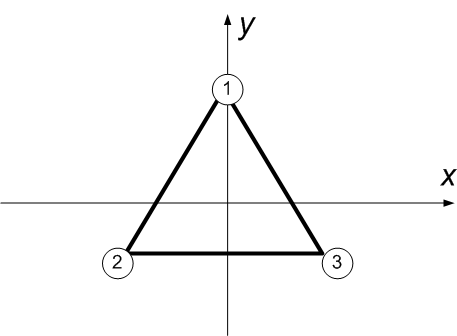
\includegraphics[width=7cm,height=6cm]{pattern}
\caption{Desired formation of three WAM-Vs\label{pattern}}
\end{center}
\end{figure}


\begin{figure}
\begin{center}
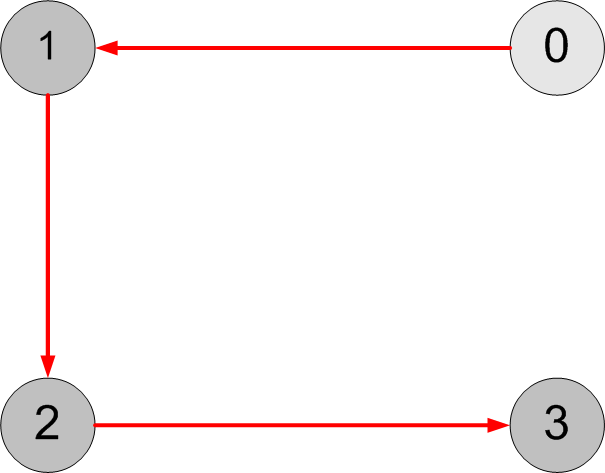
\includegraphics[width=5cm,height=5cm]{comm2}
\caption{Communication digraph\label{commd}}
\end{center}
\end{figure}


\begin{figure}

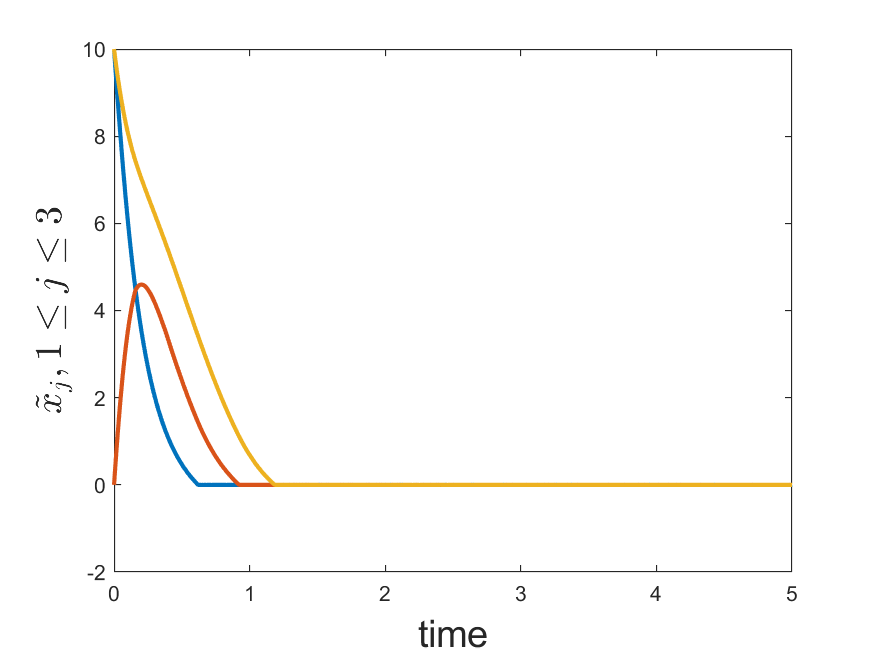
\includegraphics[width=7cm,height=5cm]{xen}
\caption{Time response of $\tilde{x}_{j}$ for $1\leq j\leq
3$\label{xed}}
\end{figure}

\begin{figure}
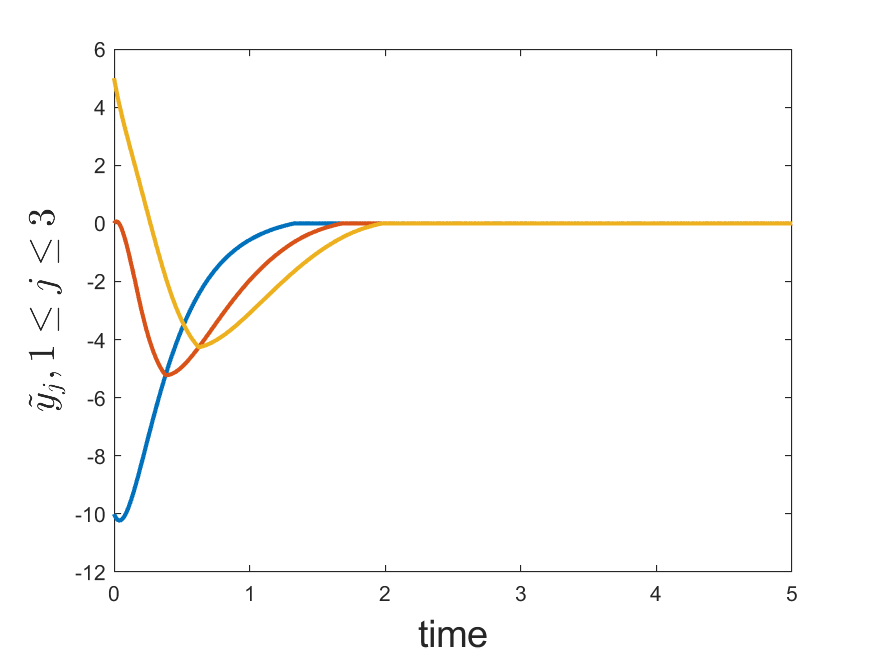
\includegraphics[width=7cm,height=5cm]{yen}
\caption{Time response of $\tilde{y}_{j}$ for $1\leq j\leq
3$\label{yed}}
\end{figure}

\begin{figure}
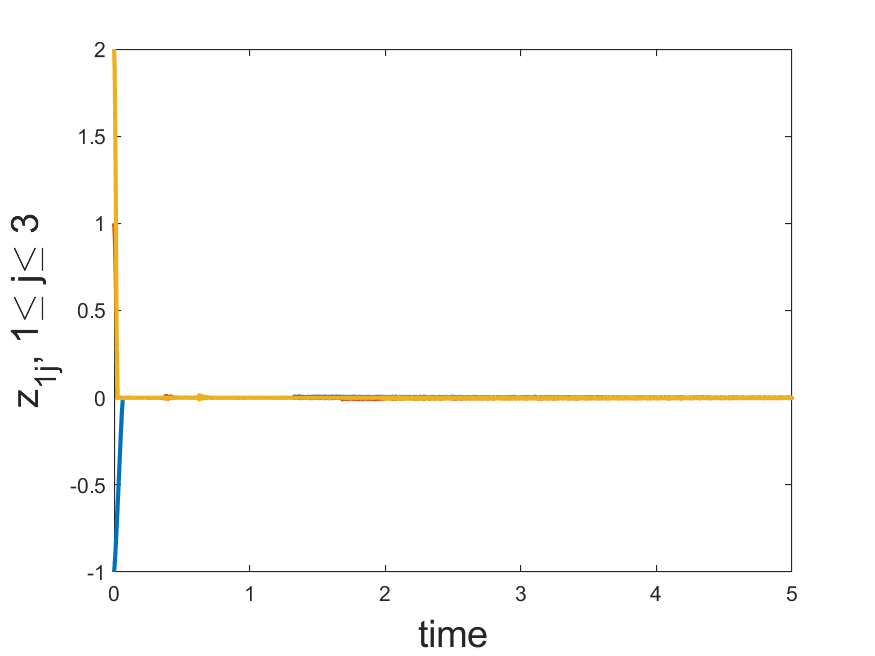
\includegraphics[width=7cm,height=5cm]{z1}
\caption{Time response of $z_{1j}$ for $1\leq j\leq
3$\label{z1}}
\end{figure}
\begin{figure}
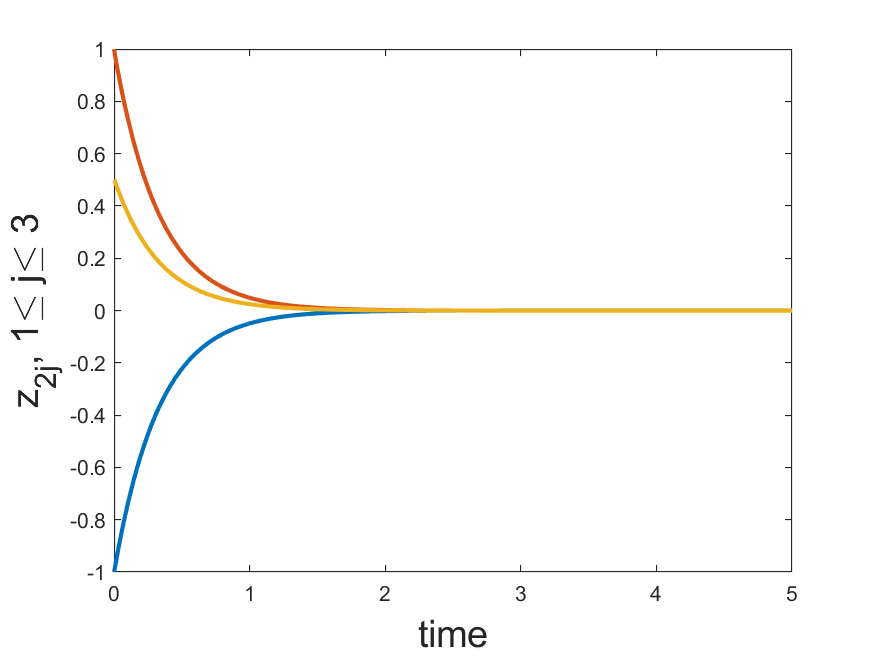
\includegraphics[width=7cm,height=5cm]{z2}
\caption{Time response of $z_{2j}$ for $1\leq j\leq
3$\label{z2}}
\end{figure}


\begin{figure}
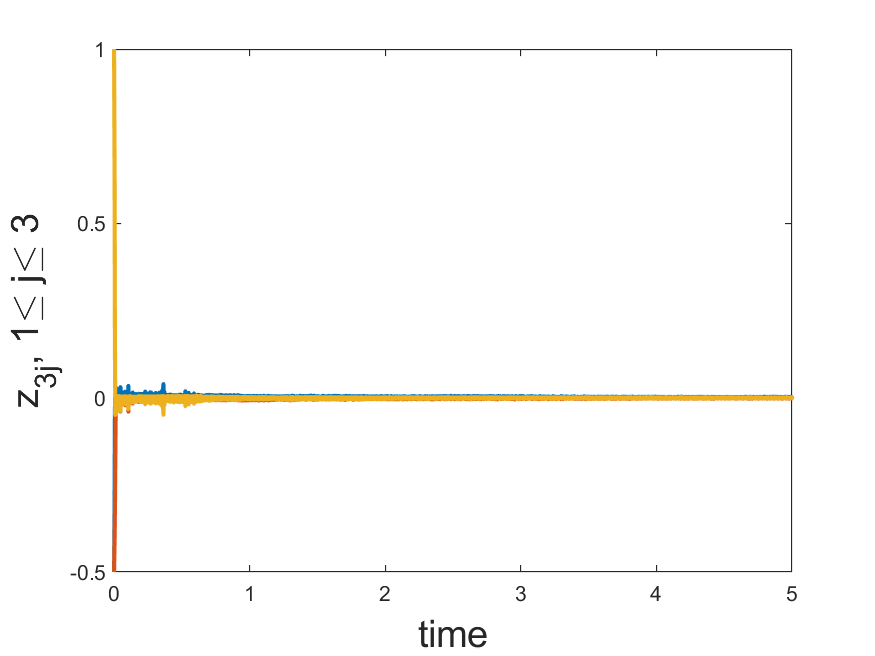
\includegraphics[width=7cm,height=5cm]{z3}
\caption{Time response of $z_{3j}$ for $1\leq j\leq
3$\label{z3}}
\end{figure}


\section{Conclusion}
\label{sec6}

In this paper, we considered formation control of
multiple uncertain WAM-Vs with a leader WAM-V. If inertia parameters are not exactly known, distributed robust tracking laws were proposed with the aid of neighbors' information. To reduce the computation load in controller design, distributed command filtered controllers were proposed. Simulation results show the effectiveness of the proposed results.

\bibliographystyle{IEEEtran}
\bibliography{bib_dong}



\end{document}
